\title{Reiknirit Bellmans og Fords ($1958$ og $1956$)}
\author{Bergur Snorrason}
\date{\today}

\begin{document}

\frame{\titlepage}

\section{Inngangur}
\env{frame}
{
    \env{itemize}
    {
        \item<1-> Hvað gerum við ef við viljum nota reinkirit Dijkstras en það mega vera neikvæðar vigtir á leggjunum.
            \item<2-> Við getum þá notað reiknirit sem er kennt við Bellman og Ford.
            \item<3-> Við þurfum þó að fórna keyrslutíma.
    }
}

\section{Lýsing}
\env{frame}
{
    \env{itemize}
    {
        \item<1-> Þetta reiknirit er að vissu leiti einfaldara en reiknirit Dijkstras.
            \item<2-> Við notum kvika bestun og svörum spurningunni ,,Hver er stysta leiðin frá $u$ til $v$ sem fer að mestu í $k$ hnúta?''.
            \item<3-> Hér táknar $u$ upphafshnútinn á meðan $v$ og $k$ eru frjálsar breytur.
            \item<4-> Látum þá $f(v, k)$ tákna systa veg frá hnútnum $u$ til hnútsins $v$ sem fer ekki í fleiri en $k$ hnúta.
            \item<5-> Til að einfalda skriftir þá skilgreinum við
            \[
            E_u = \{v \in V:\, (u, v) \in E\}
        \]
            og
            \[
            E^v = \{u \in V:\, (u, v) \in E\}.
                \]
                \item<6-> Við fáum að
    }
    \onslide<7->
    {
        \[
            f(v, k) = \left \{
            \env{array}
            { {l l}
                0, & \text{ef $u = v$ og $k = 0$}\\
                \infty, & \text{ef $u \neq v$ og $k = 0$}\\
                \min(f(v, k - 1), & \\
                        \ \min_{u \in E^v} w((u, v)) + f(u, k - 1)), & \text{annars.}
            }
            \right .
        \]
    }
}

\section{Atriði varðandi útfærslu}
\env{frame}
{
    \env{itemize}
    {
        \item<1-> Við munum leysa þetta með neðansækinni kvikri bestun.
            \item<2-> Gerum ráð fyrir að taflan sem við notum fyrir minnun hafi dálk sem svari til $k$ breytunnar.
            \item<3-> Þá er hver staða aðeins háð stöðum í röðinni fyrir ofan sig.
            \item<4-> Við notum því aðeins síðustu línu fylkisins þegar við fyllum inn í töfluna.
            \item<5-> Því má geyma tvívíða fylkið sem einvítt fylki.
    }
}

\section{Atriði varðandi neikvæðar rásir}
\env{frame}
{
    \env{itemize}
    {
        \item<1-> Við erum ekki búin þegar við höfum reiknað öll gildin á $f(v, k)$.
            \item<2-> Hvað með neikvæðar rásir?
            \item<3-> Takið fyrst eftir að ef það er ekki neikvæð rás í netinu þá heimsækir systi vegur milli hnúta engan hnúta tvisvar.
            \item<4-> Einnig er ekki nóg að það sé neikvæð rás í netinu heldur þarf að vera hægt að komast í hana frá upphafshnútnum
            og svo má vera að það sé ekki hægt að komast frá rásinni í alla aðra hnúta.
            \item<5-> Við getum einfaldlega prófað að lengja vegina um $V - 1$ hnúta í viðbót.
            \item<6-> Ef vegalengdin styttist einhverntíman þá er betra að heimsækja einhvern hnút oftar en einu sinni,
            sem þýðir að það sé neikvæð rás á leiðinni.
    }
}

\section{Sýnidæmi}
\env{frame}
{
    \env{center}
    {
        \env{tikzpicture}
        { [scale = 0.75]
            \onslide<all:2->{\node[draw, circle] (1) at (2, 2) {\tiny $1$};}
            \onslide<all:1>{\node[draw, circle, blue] (1) at (2, 2) {\tiny $1$};}

            \onslide<all:1-3, 6->{\node[draw, circle] (2) at (2, 4) {\tiny $2$};}
            \onslide<all:4, 5>{\node[draw, circle, blue] (2) at (2, 4) {\tiny $2$};}

            \onslide<all:1, 3->{\node[draw, circle] (3) at (2, 0) {\tiny $3$};}
            \onslide<all:2>{\node[draw, circle, blue] (3) at (2, 0) {\tiny $3$};}

            \onslide<all:1-2, 5->{\node[draw, circle] (4) at (4, 3) {\tiny $4$};}
            \onslide<all:3, 4>{\node[draw, circle, blue] (4) at (4, 3) {\tiny $4$};}

            \onslide<all:1, 4->{\node[draw, circle] (5) at (4, 1) {\tiny $5$};}
            \onslide<all:2, 3>{\node[draw, circle, blue] (5) at (4, 1) {\tiny $5$};}

            \onslide<all:1-3, 6-7, 9->{\node[draw, circle] (6) at (6, 2) {\tiny $6$};}
            \onslide<all:4, 5, 8>{\node[draw, circle, blue] (6) at (6, 2) {\tiny $6$};}

            \onslide<all:1-3, 6->{\node[draw, circle] (7) at (6, 4) {\tiny $7$};}
            \onslide<all:4, 5>{\node[draw, circle, blue] (7) at (6, 4) {\tiny $7$};}

            \onslide<all:1-4, 7-8, 10->{\node[draw, circle] (8) at (6, 0) {\tiny $8$};}
            \onslide<all:5, 6, 9>{\node[draw, circle, blue] (8) at (6, 0) {\tiny $8$};}

            \onslide<all:1-5, 8-9, 11->{\node[draw, circle] (9) at (8, 2) {\tiny $9$};}
            \onslide<all:6, 7, 10>{\node[draw, circle, blue] (9) at (8, 2) {\tiny $9$};}



            \path[draw, thick, <-] (1) -- (2); \node[fill = white] at (2,3) {\tiny $1$};
            \path[draw, thick, <-] (2) -- (4); \node[fill = white] at (3,3.5) {\tiny $9$};
            \path[draw, thick, <->] (4) -- (5); \node[fill = white] at (4,2) {\tiny $1$};
            \path[draw, thick, ->] (3) -- (5); \node[fill = white] at (3,0.5) {\tiny $2$};
            \path[draw, thick, ->] (1) -- (3); \node[fill = white] at (2,1) {\tiny $-4$};
            \path[draw, thick, ->] (4) -- (6); \node[fill = white] at (5,2.5) {\tiny $3$};
            \path[draw, thick, ->] (6) -- (8); \node[fill = white] at (6,1) {\tiny $5$};
            \path[draw, thick, ->] (8) -- (9); \node[fill = white] at (7,1) {\tiny $1$};
            \path[draw, thick, <-] (7) -- (9); \node[fill = white] at (7,3) {\tiny $1$};
            \path[draw, thick, <-] (6) -- (9); \node[fill = white] at (7,2) {\tiny $-7$};
            \path[draw, thick, <->] (1) -- (5); \node[fill = white] at (3,1.5) {\tiny $3$};
            \path[draw, thick, ->] (4) -- (7); \node[fill = white] at (5,3.5) {\tiny $8$};
        }
        % view this array in fullscreen.
            \[
            \env{array}
        { {r | r r r r r r r r r}
            k & 1 &      2 &      3 &      4 &      5 &      6 &      7 &             8 &             9\\
                \hline
                \onslide<all:1->  {0 & \color{blue} 0 &          \infty &          \infty &          \infty &          \infty &         \infty &          \infty &          \infty &          \infty}\\
                \onslide<all:2->  {1 &              0 &          \infty & \color{blue} -4 &          \infty & \color{blue}  3 &         \infty &          \infty &          \infty &          \infty}\\
                \onslide<all:3->  {2 &              0 &          \infty &              -4 & \color{blue}  4 & \color{blue} -2 &         \infty &          \infty &          \infty &          \infty}\\
                \onslide<all:4->  {3 &              0 & \color{blue} 13 &              -4 & \color{blue} -1 &              -2 & \color{blue} 7 & \color{blue} 12 &          \infty &          \infty}\\
                \onslide<all:5->  {4 &              0 & \color{blue}  8 &              -4 &              -1 &              -2 & \color{blue} 2 & \color{blue}  7 & \color{blue} 12 &          \infty}\\
                \onslide<all:6->  {5 &              0 &               8 &              -4 &              -1 &              -2 &              2 &               7 & \color{blue}  7 & \color{blue} 13}\\
                \onslide<all:7->  {6 &              0 &               8 &              -4 &              -1 &              -2 &              2 &               7 &               7 & \color{blue}  8}\\
                \onslide<all:8->  {7 &              0 &               8 &              -4 &              -1 &              -2 & \color{blue} 1 &               7 &               7 &               8}\\
                \onslide<all:9->  {8 &              0 &               8 &              -4 &              -1 &              -2 &              1 &               7 &  \color{blue} 6 &               8}\\
                \onslide<all:10-> {9 &              0 &               8 &              -4 &              -1 &              -2 &              1 &               7 &               6 &   \color{red} 7}\\
        }
        \]
    }
}

\section{Útfærsla}
\env{frame}
{
    \selectcode{code/bellman-ford.cpp}{9}{24}
}

\section{Tímaflækja}
\env{frame}
{
    \env{itemize}
    {
        \item<1-> Sjáum að í fyrri hluta reikniritsins ýtrum við í gegnum alla leggi og allar hnúta $(V - 1)$-sinnum.
        \item<2-> Tímaflækjan á þeim hluta er því $\mathcal{O}($\onslide<3->{$E \cdot V$}$)$.
        \item<4-> Seinni hlutinn er svo að ítra yfir nákvæmlega það sama, svo tímaflækja þar er eins.
        \item<5-> Því fæst að reikniritið er í heildina $\mathcal{O}($\onslide<6->{$E \cdot V$}$)$.
        \item<7-> Þetta er töluvert verra en reiknirit Dijkstras (svipað og að fara úr $\mathcal{O}(n \log n)$ í $\mathcal{O}(n^2)$).
    }
}

\section{Lítil bæting á keyrsluhraða}
\env{frame}
{
    \env{itemize}
    {
        \item<1-> Tökum eftir að það er ekki uppfært gildi í hnút $v$ eftir legg $(u, v)$ nema að $u$ hafi verið uppfært í umferðinni áður.
        \item<2-> Í sýnidæminu svara þetta til bláu gildanna.
        \item<3-> Við getum notað þetta til að bæta keyrlsuhraðann, án þess þó að bæta tímaflækjuna.
    }
}

\section{Útfærsla}
\env{frame}
{
    \selectcode{code/bellman-ford-faster.cpp}{9}{22}
}

\section{Bæting}
\env{frame}
{
    \env{center}
    {
        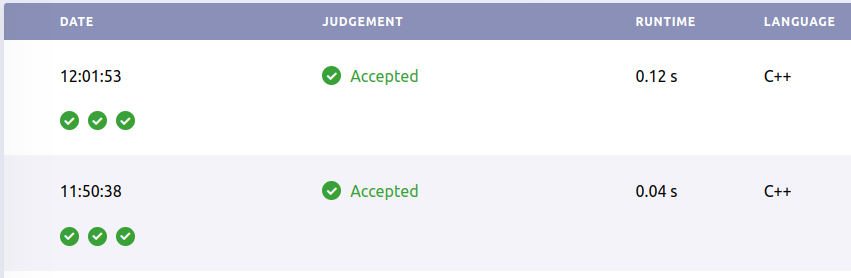
\includegraphics[scale = 0.35]{fig/ex.png}
    }
}

\section{Frekari bætingar}
\env{frame}
{
    \env{itemize}
    {
        \item<1-> Það ber að nefna að ef við notum forgangsbiðröð í stað þess að nota biðröð fáum við reiknirit Dijkstras.
        \item<2-> Ein lítil bæting í viðbót er að geyma hnútanna sem við eigum eftir að uppfæra á hlaða.
        \item<3-> Þetta getur sparað vinna, þá aðallega þegar forgangsbiðröðin er nærri tóm.
        \item<4-> Það þarf þó að passa að setja aldrei hnút í biðröðina tvisvar.
        \item<5-> Í versta falli er þessi ,,bæting'' jafn hröð og fyrri bætingin, og mögulega aðeins hægari.
        \item<6-> Hún virkar þó sérstaklega vel á slembin net.
    }
}

\section{Útfærsla}
\env{frame}
{
    \selectcode{code/bellman-ford-sometimes-faster.cpp}{9}{29}
}

\section{Þessi glæra er viljandi auð}
\env{frame}
{
}

\end{document}
